\chapter{Diseño de la Aplicación}
\label{cap:disenoDeLaAplicacion}

\begin{FraseCelebre}
\begin{Frase}
  En esencia, hay dos enfoques fundamentales del diseño: el ideal artístico de expresarse a sí mismo y el ideal de la ingeniería de resolver un problema para un cliente.
\end{Frase}
\begin{Fuente}
  Jakob Nielsen
\end{Fuente}
\end{FraseCelebre}

\section{Introducción}

El análisis, la planificación y el diseño de un proyecto software constituyen etapas fundamentales dentro de su ciclo de desarrollo (\cite{Pressman_2010}). Un enfoque basado en un análisis exhaustivo de los requisitos, junto con un diseño centrado en las necesidades del usuario, no solo permite garantizar el cumplimiento de los objetivos funcionales del sistema, sino que también contribuye a reducir la aparición de errores, optimizar los costes de desarrollo y facilitar tanto el mantenimiento como las futuras actualizaciones de la aplicación.

En este contexto, el diseño puede entenderse como un factor clave para la incorporación de calidad al producto software. Tal y como señalan \cite{Olsina_Lafuente_Rossi_2001}, la calidad de una aplicación no es un atributo único, sino el resultado de la combinación de múltiples características. Estos autores proponen un \textit{árbol de requerimientos de calidad} que identifica los principales elementos sobre los que es necesario incidir a lo largo del desarrollo del proyecto, especialmente en el caso de aplicaciones web, donde aspectos como la usabilidad, la eficiencia o la confiabilidad adquieren un papel especialmente relevante.

\begin{figure}[ht]
\centering
\hspace*{-1.2cm}
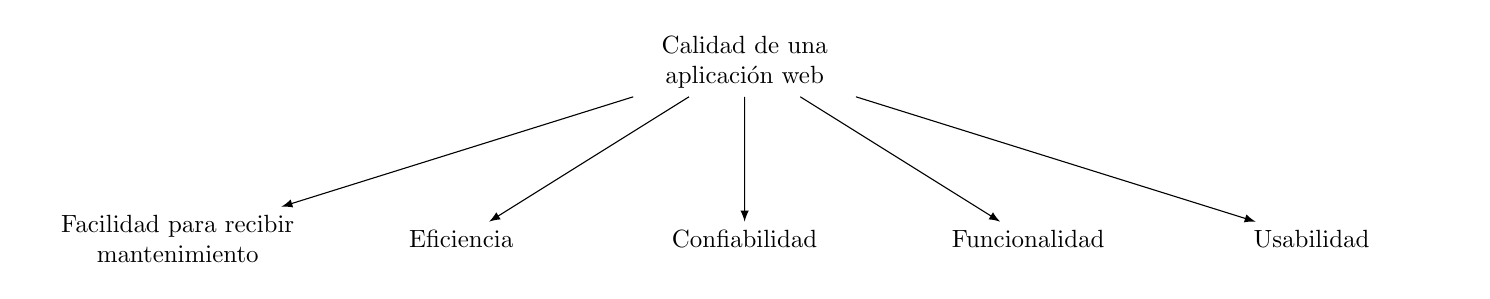
\begin{tikzpicture}[
    grow=down,
    level 1/.style={
        level distance=2.5cm,
        sibling distance=4cm,
        font=\normalsize,
        align=center
    },
    edge from parent/.style={draw,-latex},
    every node/.style={
        text width=4cm,
        align=center
    },
    scale=0.9,
    transform shape
]

\node {Calidad de una aplicación web}
    child { node {Facilidad para recibir mantenimiento} }
    child { node {Eficiencia} }
    child { node {Confiabilidad} }
    child { node {Funcionalidad} }
    child { node {Usabilidad} };

\end{tikzpicture}
\caption{Árbol de los requisitos de calidad para una aplicación web}
\end{figure}

Atendiendo a estos principios, el diseño de la aplicación se aborda en este capítulo desde una perspectiva multidimensional. En primer lugar, se definen las funcionalidades del sistema a partir de un análisis detallado de los usuarios finales y de los objetivos del proyecto, seleccionando aquellas capacidades que resultan esenciales para satisfacer los requisitos previamente identificados. De forma paralela, se plantea el diseño de la arquitectura técnica del sistema, describiendo sus distintos componentes y justificando la selección de las tecnologías empleadas para su implementación, siempre teniendo en cuenta criterios de eficiencia, confiabilidad y facilidad de mantenimiento.

Finalmente, se desarrolla el diseño de la interfaz y de la experiencia de usuario (UI/UX), prestando especial atención a la forma en que se presentan las estadísticas, a los elementos gráficos utilizados y a la estructura general de la aplicación desde el punto de vista del usuario. En esta fase, la usabilidad se convierte en el eje central del diseño, con el objetivo de garantizar una interacción intuitiva, clara y satisfactoria con el sistema.

\section{Análisis de requisitos}

El primer paso de nuestro diseño será identificar los requisitos que el software debe suplir. Este análisis sirve de base para todo el diseño, ya que establece qué se debe implementar, con qué eficiencia, y quién es nuestro público objetivo. 

A partir del análisis de requisitos recogido en el Apéndice \ref{cap:SRS}, se definen en esta sección las funcionalidades que conforman la aplicación. Dichas funcionalidades responden directamente a los requisitos funcionales identificados en la SRS y constituyen el núcleo del sistema desde el punto de vista del usuario final.

El diseño funcional se ha orientado a proporcionar información relevante, clara y actualizada sobre la actividad de los usuarios en el juez \aer, así como a introducir mecanismos de motivación adicionales mediante la gamificación. Para ello, las funcionalidades se agrupan en cuatro bloques principales: estadísticas de usuario, estadísticas de ejercicios, sistema de logros y tabla de clasificación.

\subsection{Estadísticas de usuario}

Una de las funcionalidades centrales del sistema es la visualización de estadísticas asociadas a cada usuario (REQ-FUN-001). Estas estadísticas permiten reflejar de manera cuantitativa el progreso y la actividad del usuario dentro del juez \textit{online}.

Entre la información mostrada se incluyen, entre otros indicadores, el número total de ejercicios resueltos, el número de envíos realizados y la tasa de aciertos. Estos datos se presentan de forma agregada y comprensible, con el objetivo de que el usuario pueda evaluar su evolución a lo largo del tiempo y detectar posibles áreas de mejora.

Las estadísticas de usuario se actualizan automáticamente cuando se producen eventos relevantes en el sistema, como la evaluación de un nuevo envío (REQ-FUN-003). De este modo, se garantiza que la información mostrada sea coherente con el estado real del sistema y no requiera ninguna acción manual por parte del usuario.

\subsection{Estadísticas de ejercicios}

Además de las estadísticas individuales, el sistema proporciona estadísticas asociadas a los ejercicios disponibles en el juez (REQ-FUN-002). Estas estadísticas se calculan de forma agregada a partir de la actividad de todos los usuarios y permiten ofrecer una visión global de cada problema.

Entre los indicadores considerados se encuentran el número de intentos realizados y el porcentaje de éxito. Esta información resulta útil para que los usuarios puedan estimar la dificultad relativa de los ejercicios, así como su popularidad dentro de la plataforma.

Al igual que ocurre con las estadísticas de usuario, las estadísticas de ejercicios se actualizan automáticamente conforme se registran nuevos envíos evaluados, garantizando la consistencia y fiabilidad de los datos mostrados.

\subsection{Sistema de logros}

Con el objetivo de incrementar la motivación y fomentar la participación activa, el sistema incorpora un sistema de logros o medallas (REQ-FUN-004). Los logros se otorgan automáticamente cuando un usuario cumple una serie de condiciones predefinidas, como alcanzar un determinado número de ejercicios resueltos.

Cada logro representa un hito alcanzado por el usuario y actúa como una recompensa simbólica que refuerza comportamientos positivos dentro del sistema. El diseño funcional del sistema de logros debe ser extensible, permitiendo la incorporación de nuevos logros en el futuro sin necesidad de modificar la lógica principal de la aplicación.

Los usuarios pueden consultar en todo momento la lista de logros obtenidos (REQ-FUN-005), accediendo a una vista específica en la que se muestran de manera clara y ordenada. Esta funcionalidad contribuye a reforzar la percepción de progreso y a mantener el interés del usuario a largo plazo.

\subsection{Tabla de clasificación}

Otra funcionalidad clave del sistema es la tabla de clasificación de usuarios (REQ-FUN-006 y REQ-FUN-007). Esta tabla ordena a los usuarios en función de su puntuación, calculada a partir de su actividad y de los logros alcanzados.

La tabla de clasificación se actualiza automáticamente cada vez que se produce un evento que afecta a la puntuación de un usuario, garantizando que la información mostrada sea siempre actual. Desde el punto de vista funcional, se permite a los usuarios consultar tanto su propia posición como la del resto de participantes, favoreciendo la comparación y la competencia.

\subsection{Compartición de estadísticas y logros}

Finalmente, el sistema contempla la posibilidad de compartir estadísticas o logros obtenidos por un usuario (REQ-FUN-008). Esta funcionalidad permite generar una imagen o enlace que represente visualmente un logro o un conjunto de estadísticas, facilitando su difusión fuera de la plataforma.

Desde el punto de vista funcional, esta característica busca aumentar la visibilidad del progreso del usuario y reforzar la motivación mediante el reconocimiento externo.

\section{Diseño del sistema de gamificación}

Como se ha establecido previamente, el objetivo de este proyecto es incorporar componentes de estadísticas y logros en el juez \textit{online} \aer para impulsar la motivación, la fidelización de los usuarios y facilitar su proceso de aprendizaje. Los elementos que se pretenden integrar se corresponden con mecánicas de juego. Por consiguiente, el proceso de diseño de estas funciones en la aplicación no consiste únicamente en añadir características aisladas, sino en aplicar de manera consciente y estructurada principios de diseño de juegos relevantes para generar experiencias que resulten atractivas y significativas para los usuarios. Este proceso se reconoce como \textbf{gamificación} (del inglés \textit{game}, juego). 

\subsection{Introducción a la gamificación}

El concepto de la gamificación ha emergido a partir de comienzos del siglo XXI como un campo interdisciplinario que combina principios de diseño de juegos, psicología motivacional y análisis de comportamiento humano para enriquecer la interacción con sistemas digitales\footnote{Se recomienda leer la siguiente presentación realizada por Amy Jo Kim en 2008, en la que se muestra claramente el panorama de la gamificación en la decada de los 2000: \url{https://es.slideshare.net/slideshow/putting-the-fun-in-functiona/300487\#1}}. En términos generales, la gamificación se define como la utilización de elementos y mecánicas de juego con el propósito de motivar a los usuarios, aumentar su participación y ayudarles a resolver problemas (\cite{Zichermann_Cunningham_2011}). En este sentido, la gamificación representa una herramienta para fomentar comportamientos deseables y no una solución mágica o independiente de contexto. Por ello, es crucial evitar prácticas de “gamificación por gamificar” que carezcan de un análisis previo sobre su pertinencia y efectos esperados. También conviene considerar la diferencia entre la motivación extrínseca (que procede de estímulos externos) e intrínseca (que procede de un deseo interno) a la hora de gamificar. Nuestro objetivo será producir una fuente de motivación extrínseca que ofrezca resultados predecibles en los usuarios, pero sea tan agradable y fluida para el usuario que parezca intrínseca. 

De forma complementaria, otros autores la describen como el enriquecimiento de software mediante características de diseño propias de los juegos, con el objetivo de generar experiencias tan atractivas y absorbentes como las que ofrecen los juegos tradicionales (\cite{Morschheuser_Hassan_Werder_Hamari_2018}). Este enfoque subraya que el diseño gamificado va más allá de la simple aplicación de recompensas superficiales y requiere integrar conocimientos sobre motivación y diseño de juegos para que las interacciones resulten realmente significativas y no solo un añadido cosmético.

Por lo tanto, se debe realizar un análisis de los usuarios (en esta sección también llamados \textit{jugadores}) y mecánicas, para determinar qué es más conveniente en el contexto dado.

\subsection{Análisis de jugadores y mecánicas}

En la sección anterior hemos destacado la importancia de la motivación extrínseca para crear un buen sistema de gamificación. Sin embargo, todo diseño de gamificación debe realizarse con el foco en el jugador. Comprender qué motiva a los jugadores es esencial para construir un sistema gamificado exitoso.

Según \cite{bartle_players_muds}, los jugadores pueden clasificarse en cuatro tipos no excluyentes, que determinan como debe diseñarse la experiencia de juego para poder fidelizarlos. Las cuatro categorías son:
\begin{itemize}
    \item Exploradores: Buscan descubrir y experimentar.
    \item Logradores (Achievers): Se enfocan en completar objetivos y acumular recompensas.
    \item Socializadores: Priorizan la interacción con otros jugadores.
    \item Competidores (Killers): Disfrutan superando a otros, incluso a costa de la colaboración. Es decir, no solo buscan ganar, si no que además buscan hacer perder a otro.
\end{itemize}

\begin{figure}
    \centering
    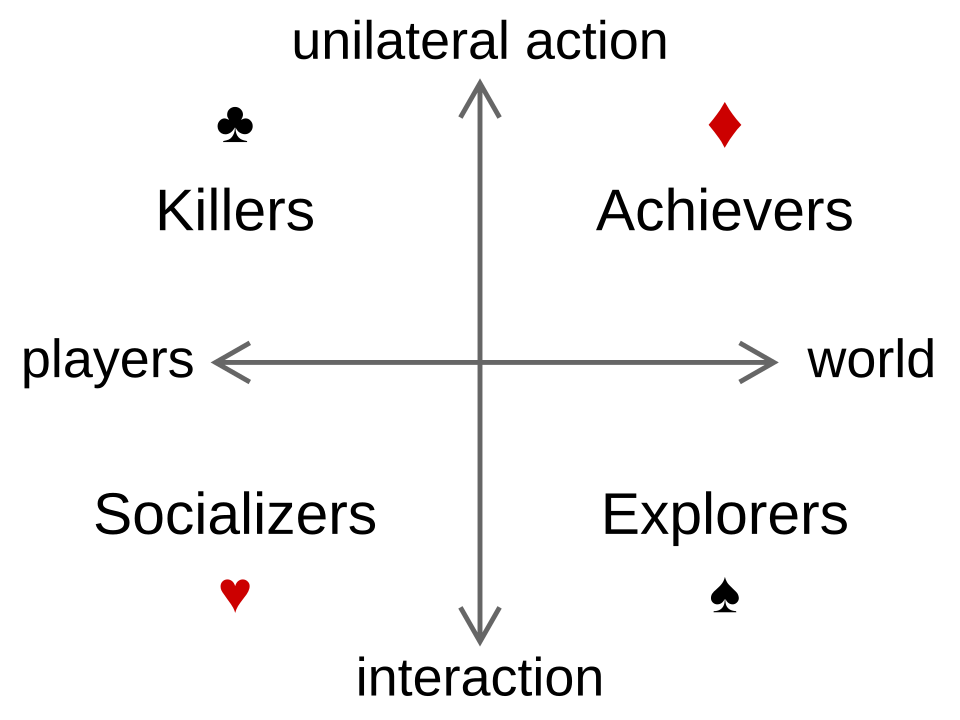
\includegraphics[width=0.5\linewidth]{Imagenes/Bitmap/Character_theory_chart.svg.png}
    \caption{Gráfico de la taxonomía de jugadores de Bartle. Se trata de una versión gráfica disponible en la página de Wikipedia correspondiente, basada en el dibujo taxonómico realizado por Bartle con ASCII en su artículo original.}
    \label{fig:Taxonomía de jugadores de Bartle}
\end{figure}

Para determinar a qué categoría pertenecen nuestros jugadores objetivo en las distintas áreas de la aplicación, se diseñó un formulario cuyos resultados se recogen en el apéndice \ref{FormularioJugadores}. El análisis de estos datos revela patrones relevantes en relación con las preferencias y motivaciones de los jugadores. A continuación, se presentan las principales implicaciones de dichos resultados para cada una de las categorías del modelo de Bartle:

\begin{enumerate}
    \item Competidores (Killers): Tal y como cabía esperar en un entorno de programación competitiva, los resultados reflejan una presencia notable de comportamientos asociados al perfil competitivo, especialmente en contextos de comparación directa y resolución de problemas de alta dificultad. El fuerte interés mostrado por las tablas de clasificación (con más del 90\% de los encuestados manifestando su deseo de aparecer en ellas), así como la preferencia por mecanismos de filtrado por nivel o tipo de problema, refuerzan esta interpretación
 No obstante, este perfil aparece de forma más limitada en aspectos relacionados con la satisfacción personal, la motivación intrínseca o el reconocimiento individual. En consecuencia, aunque resulta imprescindible incorporar mecánicas competitivas como rankings y comparaciones entre usuarios, estas no deben dominar el diseño global del sistema de gamificación.
    
    \item Logradores (Achievers): El perfil de logrador es el más consistente a lo largo de los distintos contextos analizados y adquiere especial relevancia en relación con la satisfacción y el progreso personal. Este comportamiento está alineado con el carácter educativo de la plataforma y con los resultados de la encuesta, donde los usuarios valoran especialmente poder visualizar su mejora a lo largo del tiempo, el número de envíos correctos o el tiempo invertido.  
Desde el punto de vista del diseño, esto justifica la implementación de un sistema variado de insignias y logros, así como estadísticas claras y detalladas que permitan a los usuarios seguir su evolución, comparar su rendimiento entre distintos periodos o lenguajes de programación y recibir retroalimentación constante sobre su progreso.
    
    \item Exploradores (Explorers): El perfil explorador destaca principalmente en los contextos de aprendizaje. Los usuarios muestran interés por descubrir nuevas estrategias, experimentar con distintos tipos de problemas o lenguajes, y obtener reconocimiento por enfoques menos convencionales. Este comportamiento se refleja, por ejemplo, en el interés por logros asociados a tipos de problemas, características específicas de los envíos o lenguajes utilizados.  
En consecuencia, el diseño del sistema de gamificación debe contemplar la inclusión de elementos que fomenten la exploración, como contenido desbloqueable o insignias especiales, incluyendo un número limitado de \textit{insignias sorpresa} o \textit{medallas misteriosas}, cuya aceptación, aunque no unánime, resulta significativa para una parte de los usuarios.
    
    \item Socializadores (Socializers): Aunque se trata del perfil menos predominante en términos generales, los socializadores aparecen en aquellos contextos en los que la colaboración contribuye al aprendizaje. Estos jugadores encuentran satisfacción en cooperar para alcanzar soluciones o en enseñar a otros. Dado que \aer no dispone de funcionalidades sociales como foros o soporte para grupos, y que el desarrollo de dichas características queda fuera del alcance de este proyecto, unido a la baja representación de este perfil, no se implementarán técnicas de gamificación específicas para este grupo, como sistemas de puntos por participación en foros.
\end{enumerate}

A partir del análisis realizado, se concluye que los usuarios de la plataforma no responden a un único perfil de jugador, sino que alternan entre distintos roles en función del contexto, predominando claramente los perfiles de logrador, competidor y explorador. En general, los jugadores muestran una preferencia marcada por mecánicas que refuercen el progreso individual, la comparación objetiva del rendimiento y el dominio del \enquote{mundo del juego}, entendido como el conjunto de habilidades y conocimientos propios de la programación competitiva, frente a la interacción social con otros usuarios.

Estas conclusiones justifican un diseño de gamificación centrado en estadísticas detalladas, retroalimentación continua, sistemas de logros significativos y tablas de clasificación segmentadas por nivel. De este modo, el sistema propuesto se alinea tanto con las motivaciones detectadas en la encuesta como con los objetivos formativos de la plataforma.

\subsection{Propuesta de diseño}

Con toda la información relevante sobre los jugadores objetivo y las mecánicas disponibles recabada, se realiza una propuesta de diseño de sistema de gamificación basada en el marco teórico MDA (\textit{Mecánicas, Dinámicas, Estética}), presentado en \cite{Zichermann_Cunningham_2011}.  Esto quiere decir que la propuesta está dividida en las mecánicas a introducir, las dinámicas deseadas de los jugadores con estas mecánicas, y el sentimiento deseado en los jugadores al interactuar con las mecánicas. 

\subsubsection{Mecánicas}

El sistema de logros es la primera de las mecánicas ideada. Para su diseño, se establecieron las siguientes directrices que se corresponden con las necesidades de los usuarios establecidas en la sección anterior: 
\begin{itemize}
    \item Simplicidad y claridad: Cada logro debe poder describirse en una o dos frases como máximo, lo que garantiza su fácil comprensión por parte de los usuarios.
    \item Permanencia: Los logros deben corresponder a acciones irreversibles o que no puedan perderse. Una vez obtenido, el usuario lo conservará de forma definitiva. Por ejemplo, no se contempla un logro por conseguir todos los logros disponibles, ya que su validez se vería comprometida al incorporarse nuevos logros en el futuro.
    \item Categorización por dificultad: Los logros se clasifican en tres niveles (Bronce, Plata y Oro) según su dificultad o relevancia. Esta jerarquía, inspirada en el sistema de medallas del ámbito deportivo, resulta intuitiva y reconocible para los usuarios, y sirve como indicador de progreso. Además, otros jueces \textit{online}, como HackerRank, ya implementan esta jerarquía de logros.
    \item Categorización por tipo de acción: Los logros también se agrupan según el aspecto que premian, como la calidad de los envíos o el uso de lenguajes de programación. Las categorías definidas son:
    \begin{itemize}
        \item Onboarding: Ayudan a los usuarios a aclimatarse con el sistema de gamificación.
        \item Número de problemas: Premian al usuario por haber resuelto una cierta cantidad de problemas.
        \item Uso de lenguajes: Premian al usuario por haber usado ciertos lenguajes.
        \item Rachas: Premian al usuario por su consistencia en diferentes aspectos.
        \item Calidad: Premian al usuario por ideas soluciones buenas.
        \item Categorías: Premian al usuario por hacer ejercicios de determinadas categorías. Las cateogrías que contemplamos son: construcciones de programación, estructuras de datos, algoritmia, matemáticas, grafos y geometría. 
    \end{itemize}
    \item Logros sorpresa: Con el objetivo de fomentar la exploración y la sensación de descubrimiento en los usuarios, especialmente en aquellos con perfiles de \textit{logrador} o \textit{explorador}, se han incluido dos logros cuya descripción no es accesible hasta que se obtienen. Estos logros no ofrecen pistas sobre cómo conseguirlos y pueden desbloquearse en cualquier momento.
\end{itemize}

En la tabla \ref{tab:logros} se detallan los logros propuestos a partir de las directrices definidas, junto con su categorización:

\begin{table}[h]
\centering
\small
\begin{tabular}{p{8cm}cc}
\toprule
\textbf{Descripción} & \textbf{Nivel} & \textbf{Categoría} \\
\midrule
Creación de una cuenta & Bronce & Onboarding \\
Realización del primer envío & Bronce & Onboarding \\
Obtención de 5 logros & Plata & Onboarding \\
Resolución de 10 problemas & Bronce & Número de problemas \\
Resolución de 50 problemas & Plata & Número de problemas \\
Resolución de 100 problemas & Plata & Número de problemas \\
Resolución de 500 problemas & Oro & Número de problemas \\
Resolución de 25 problemas en C & Oro & Uso de lenguajes \\
Resolución de 25 problemas en C++ & Oro & Uso de lenguajes \\
Resolución de 25 problemas en Java & Oro & Uso de lenguajes \\
Haber realizado envíos con 3 lenguajes diferentes & Plata & Uso de lenguajes \\
Consecución de una racha de 5 envíos aceptados a la primera & Oro & Rachas \\
Realización de envíos en 7 días consecutivos & Bronce & Rachas \\
Resolución de un problema en el primer intento & Bronce & Calidad \\
Envío correcto dentro del 25\% de soluciones más rápidas para un problema & Plata & Calidad \\
Resolución de un problema de cada categoría & Oro & Categorías \\
Envío correcto que iguale o mejore el tiempo de ejecución récord para un problema & Oro & Calidad (sorpresa) \\
Realización de envíos en cada franja horaria & Plata & Rachas (sorpresa) \\
\bottomrule
\end{tabular}
\caption{Logros propuestos}
\label{tab:logros}
\end{table}

La distribución final de los logros queda establecida en 5 de nivel \textit{Bronce}, 6 de nivel \textit{Plata} y 7 de nivel \textit{Oro}. Esta proporción garantiza un equilibrio en la progresión del usuario, al tiempo que diversifica las categorías de logros según su tipo. Asimismo, se han incluido solo dos logros sorpresa, una decisión que busca satisfacer, en la mayor medida posible, las preferencias de los usuarios encuestados, cuyas opiniones sobre este aspecto estuvieron divididas.

La siguiente mecánica a definir es el tema de las estadísticas. Dispondremos tanto de estadísticas de cada usuario, como de cada ejercicio. 

Para los usuarios se han ideado las siguientes estadísticas, considerandolas informativas para entender rápidamente el nivel de experiencia y conocimiento de un determinado usuario, o para servir de referencia a la hora de intentar obtener ciertos logros:

\begin{enumerate}
    \item Número de problemas resueltos: Total acumulado de ejercicios completados con éxito.
    \item Posición en la tabla de clasificación global: Ubicación del usuario en el ranking general de la plataforma, basada en sus puntos de experiencia.
    \item Proporción de veredictos obtenidos en envíos.
    \item Evolución temporal de envíos realizados: 
    \begin{itemize}
        \item Visualización de los envíos realizados cada día.
        \item Racha actual de envíos: Número actual de días consecutivos con al menos un envío.
        \item Racha máxima: Mayor número de días consecutivos con envíos registrados en el historial del usuario.
    \end{itemize}
    \item Puntos de experiencia (XP) y nivel de dominio a lo largo del tiempo.
    \item Proporción de lenguajes de programación utilizados.
\end{enumerate}
Se eliminarían además las estadísticas actualmente existentes de número de problemas intentados, número de envíos totales realizados, y número de envíos AC. En el caso de los dos primeros debido a que no responden a ninguna necesidad específica de un estudiante que quiere conocer su estado en el sistema, sobretodo en su representación númerica actual. Serían remplazadas por las estadísticas del punto 4, que además de dar la información sobre cantidad de envíos realizados lo representan y comparan en el tiempo, aplicandolo a una necesidad real (entender el progreso en el tiempo). Por otro lado el número de envíos AC es redundante cuando ya existe una estadística que indica el número de problemas resueltos y otra que indica la proporción de veredictos obtenidos.

El sistema de puntos implementado se basa en el modelo de puntos de experiencia (XP), el cual se diferencia de otros sistemas de puntos por cumplir tres condiciones fundamentales:

\begin{itemize}
    \item No monetizable: Los puntos de experiencia no pueden canjearse por recompensas ni utilizarse como moneda dentro del sistema. Su función es exclusivamente indicativa del progreso del usuario.
    \item Acumulación por actividad: Los usuarios obtienen XP por todas las acciones relevantes realizadas en la plataforma, específicamente por:
    \begin{itemize}
        \item Envíos de soluciones.
        \item Desbloqueo de logros.
    \end{itemize}
    \item Incremento permanente: Los puntos de XP solo pueden aumentar; nunca decrecen, lo que garantiza un progreso constante y sin penalizaciones.
\end{itemize}

Para facilitar la visualización del progreso, se introduce el concepto de \textbf{niveles de dominio}, que asignan un título al usuario según el rango de XP acumulado. Estos niveles permiten una comprensión inmediata de la posición del usuario dentro del sistema y fomentan la motivación mediante metas claras.

Los niveles de dominio establecidos se detallan en la Tabla~\ref{tab:niveles_dominio}.

\begin{table}[h]
\centering
\small
\begin{tabular}{cc}
\toprule
\textbf{Nivel de dominio} & \textbf{Rango de XP} \\
\midrule
Aprendiz     & 0 - 100 XP \\
Competente   & 101 - 500 XP \\
Hábil        & 501 - 1,000 XP \\
Especialista & 1,001 - 2,000 XP \\
Maestro      & Más de 2,000 XP \\
\bottomrule
\end{tabular}
\caption{Niveles de dominio según puntos de experiencia (XP)}
\label{tab:niveles_dominio}
\end{table}

Está planteado de tal manera que sea relativamente fácil abandonar los primeros niveles, pero la progresión sea más compleja con el tiempo. Por ejemplo, para pasar de aprendiz a competente se necesitan solo 100 puntos, mientras que para pasar de especialista a maestro se necesitan 1000. 
El sistema de XP permite generar una tabla de clasificación con dos vistas complementarias:

\begin{itemize}
    \item Clasificación global: Muestra la posición del usuario en relación con todos los participantes del sistema.
    \item Clasificación por nivel: Permite comparar el desempeño del usuario con otros usuarios que compartan su mismo nivel de dominio.
\end{itemize}

Este diseño fomenta la interacción competitiva entre los usuarios, al tiempo que ofrece una recompensa\textbf{ }tangible por interactuar con el sistema. Además, al vincularse directamente con el desbloqueo de logros, el sistema refuerza la sensación de progreso y logro personal.

Una característica importante a tener en cuanta tanto en el diseño como la evaluación de un sistema de gamificación es el problema de \textbf{la superación del jefe final}. Este problema se refiere a cuando un sistema de gamificación, sobretodo uno que se introduce en en un sistema ya existente con años de experiencia como es \aer, se vuelve redundante porque un número considerable de usuarios obtienen el máximo nivel de dominio, todos los logros, etc. Se pierde la fuente de motivación extrínseca y se inituliza el esfuerzo invertido en el sistema. Para evitar esto, todas las mecánicas del sistema de gamificación deben ser fácilmente extensibles. 
En nuestro caso, las estadísticas no cuentan con un \enquote{nivel máximo} y por lo tanto no corren riesgo de volverse obsoletas, ya que su único objetivo es mostrarle su situación al usuario, no evaluarle o recompensarle por ésta. Por otro lado, el sistema de logros es facilmente extensible añadiendo nuevos logros que cumplan las condiciones de diseño anteriormente definidas. Por ejemplo, podrían añadirse nuevos logros que recompensen la cantidad de ejercicios resueltos según se añadan más ejercicios a la plataforma. Finalmente, los niveles de dominio del sistema de puntos podrían ser reasignados a cantidades de XP diferentes, o definirse un nuevo nivel con su rango de XP correspondiente.

 \subsubsection{Dinámicas}
En esta sección profundizamos en una de las categorías mencionadas previamente, pero no desarrollada: la bienvenida (\textit{onboarding}). Esta etapa se centra en técnicas diseñadas para guiar al usuario en su primer contacto con el sistema, evitando la sobrecarga de información y previniendo la sensación de desorientación. Los logros resultan una herramienta especialmente efectiva para este propósito, ya que actúan como indicadores interactivos\ que orientan al usuario sobre las acciones más relevantes y sus beneficios.
Por ejemplo, el logro otorgado al \textit{crear una cuenta} cumple tres objetivos fundamentales:
\begin{enumerate}
    \item Introducir la existencia del sistema de logros.
    \item Mostrar al usuario dónde puede consultar sus logros.
    \item Demostrar que los logros otorgan puntos de experiencia (XP).
\end{enumerate}
Mediante este enfoque, el usuario aprende de manera práctica y progresiva\, sin necesidad de explicaciones teóricas. Además, la obtención de este logro inicial incluye una recompensa en XP, lo que evita que el usuario comience con 0 XP\ en la tabla de clasificación. Esto previene posibles sentimientos de inferioridad o desmotivación al compararse con otros usuarios más avanzados.
El siguiente logro, \enquote{Realización del primer envío}, refuerza este aprendizaje al indicar claramente cuál es el siguiente paso en su interacción con el sistema. De este modo, se fomenta la exploración autónoma y se facilita la comprensión de las mecánicas básicas.

A continuación, se detalla la asignación de XP según las acciones realizadas por el usuario. La distribución de puntos, presentada en la Tabla~\ref{tab:sistema-puntos}, ha sido diseñada para:
\begin{itemize}
    \item Reconocer todas las acciones relevantes (incluyendo los intentos no aceptados).
    \item Garantizar que las recompensas se perciban como significativas.
    \item Dificultar la obtención fraudulenta de XP, evitando que el sistema sea explotado de manera tediosa o artificial.
\end{itemize}

\begin{table}[h]
\centering
\small
\begin{tabular}{cc}
\toprule
\textbf{Acción} & \textbf{XP recibido} \\
\midrule
Envío no aceptado            & 1 XP \\
Envío aceptado               & 15 XP \\
Obtención de logro de bronce & 20 XP \\
Obtención de logro de plata  & 40 XP \\
Obtención de logro de oro    & 60 XP \\
\bottomrule
\end{tabular}
\caption{Acciones y recompensas en XP}
\label{tab:sistema-puntos}
\end{table}

Sin embargo, según el sistema continúe creciendo y ante la posibilidad de que se redistribuyan o creen niveles de dominio, las recompensas podrán ser editadas.

\subsubsection{Estética}
El diseño del sistema de logros, estadísticas y puntos de experiencia (XP) busca evocar en los usuarios dos sensaciones fundamentales, alineadas con los principios de la \textbf{conciencia situacional} y la \textbf{motivación extrínseca}. Estas emociones no solo mejoran la experiencia del usuario, sino que también refuerzan su compromiso a largo plazo con la plataforma.

La conciencia situacional se refiere a la capacidad del usuario para comprender su posición actual dentro del sistema, así como las acciones necesarias para mejorar (\cite{Endsley_Jones_2012}.) En este contexto, se logra mediante:
\begin{itemize}
    \item Retroalimentación visual clara: Las estadísticas y los niveles de dominio proporcionan una imagen inmediata del progreso del usuario, permitiéndole identificar sus fortalezas y áreas de mejora.
    \item Objetivos definidos: Los logros actúan como hitos tangibles que guían al usuario hacia metas concretas, facilitando la planificación de su progreso.
    \item Contexto relevante: La información presentada (como la tabla de clasificación y los niveles de dominio) está directamente vinculada a los objetivos del usuario, evitando la sobrecarga de datos irrelevantes.
\end{itemize}

Esta conciencia permite al usuario no solo saber dónde se encuentra, sino también comprender qué acciones debe tomar para avanzar, fomentando una experiencia de aprendizaje autónoma y significativa.

La motivación extrínseca en este sistema se centra en el reconocimiento social y el aumento de estatus. Las estrategias clave incluyen:
\begin{itemize}
    \item Logros y medallas: Actúan como símbolos de estatus que el usuario puede mostrar, generando un sentido de orgullo y pertenencia dentro de la comunidad.
    \item Tabla de clasificación: Fomenta la competencia saludable, especialmente en usuarios con perfiles hipercompetitivos, quienes buscan destacar incluso sin recompensas tangibles.
    \item Recompensas progresivas: Los puntos de experiencia (XP) y los niveles de dominio ofrecen una sensación de avance constante, reduciendo el riesgo de que el usuario dependa exclusivamente de "victorias" puntuales para mantener su motivación.
\end{itemize}

En conjunto, estas estrategias buscan crear una experiencia donde los usuarios se sientan capaces, reconocidos y motivados, equilibrando el deseo de superación personal con el disfrute del proceso.

\section{Diseño de la interfaz}
El primer paso para el diseño de la interfaz, es establecer los parámetros que guiarán el diseño de la interfaz, es decir, la guía de estilo. Los elementos de la guía de estilos se han elegido con la idea de mantener consistencia visual con la aplicación actual de acepta el reto, a la vez que se respetan las necesidades de contraste y accesibilidad:
\begin{enumerate}
    \item Para la paleta de colores se han seleccionado 8 colores distintos: 3 tonos azules originarios de \aer, donde sirven para indicar selecciones, títulos o menús, un tono claro y un tono oscuro que pueden servir para color del fondo de la página y color de la letra o viceversa según qué tema se esté utilizando, y 3 tonos rojos obtenidos a partir de los tonos azules para representar situaciones de peligro o como color de resalte. 
    \item La tipografía es la misma que en \aer: Open Sans\footnote{\url{https://fonts.google.com/specimen/Open+Sans}}, tanto para el texto general como para títulos.
    \item En cuanto a la iconografía, mantendremos la misma que en \aer. Se tratan de los iconos de Font Awesome\footnote{\url{https://fontawesome.com/v3/}}, los cuales son escalables y tienen una licencia libre. 
\end{enumerate}

\begin{figure}
    \centering
    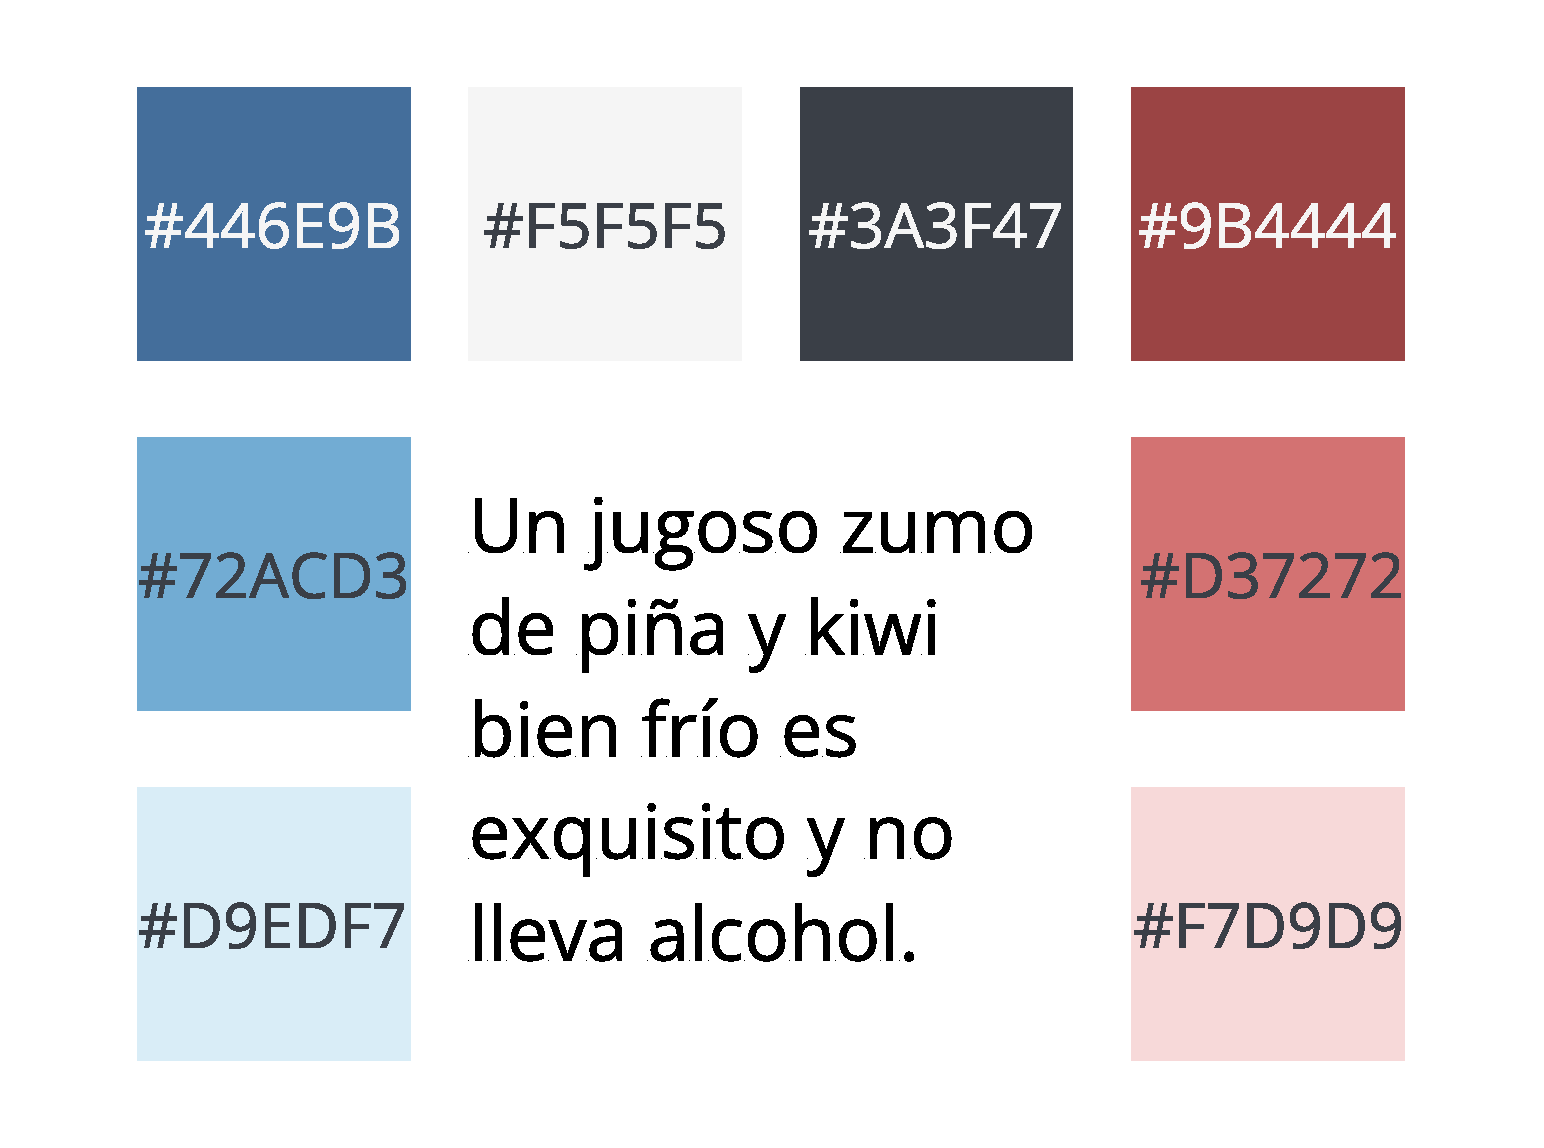
\includegraphics[width=0.5\linewidth]{Imagenes/Vectorial/Guía de estilos.pdf}
    \caption{Colores y tipografía seleccionados para la guía de estilos}
    \label{fig:guiaEstilos}
\end{figure}

En cuanto a los elementos de la interacción humano-máquina, tendremos en cuenta las heurísticas presentadas en \cite{Nielsen_1994}. En específico para nuestra aplicación son importantes la visibilidad del estado del sistema, la equivalencia entre el sistema y el mundo real, y una representación de la información que simplifique el reconocimiento de los usuarios de la información, en vez de apelar a su memoria. 

Manteniendo las heurísticas en mente, es hora de definir tanto las pantallas de nuestro sistema como su colocación de elementos para facilitar el uso (UX). Para ello, se han realizado una serie de \textit{wireframes}, una por cada pantalla de la aplicación. Las pantallas de la aplicación son:
\begin{itemize}
    \item Inicio
    \item Estadísticas de usuario
    \begin{itemize}
        \item Estadísticas
        \item Medallero
    \end{itemize}
    \item Estadísticas de un ejercicio
    \item Tabla de clasificación
\end{itemize}

TO DO : WIREFRAMES UX

TO DO: REPRESENTACIÓN DE LA INFORMACIÓN, DASHBOARDS

TO DO: DISEÑO DE LAS PLACAS DE LOGROS

\section{Arquitectura del sistema}

El diseño de la arquitectura del sistema ha sido ideado atendiendo a los requisitos no funcionales definidos para la aplicación en el apéndice \ref{cap:SRS}. En concreto, los requisitos de rendimiento (REQ-NF-001) y fiabilidad de los datos (REQ-NF-002) exigen la selección de tecnologías eficientes y robustas, capaces de garantizar un procesamiento ágil y una gestión segura de la información. Por otro lado, el requisito de usabilidad (REQ-NF-003) subraya la necesidad de implementar una interfaz y experiencia de usuario no solo intuitiva y personalizable, sino también mantenible y escalable a largo plazo.

Tras el análisis comparativo de las tecnologías disponibles, detallado en el capítulo~\ref{cap:estadoDelArteDeTecnologias}, se ha decidido adoptar un \textit{stack} tecnológico compuesto por React, Node.js y Redis para el desarrollo del \textit{frontend}, \textit{backend} y gestión de datos, respectivamente. Esta elección responde a las siguientes ventajas clave:

\begin{itemize}
    \item React: Su capacidad para construir interfaces de usuario dinámicas y reactivas lo convierte en una herramienta idónea para el proyecto. El modelo basado en componentes no solo facilita la reutilización de código, sino que también optimiza la gestión del estado de la aplicación. Esto es especialmente relevante para cargar y visualizar datos en tiempo real, evitando recargas completas de página y reduciendo los tiempos de espera.

    \item Node.js: Destaca por su arquitectura orientada a eventos, que permite manejar operaciones asíncronas de manera eficiente. Esta característica es fundamental para garantizar un \textit{backend} escalable y capaz de procesar múltiples solicitudes concurrentes sin degradar el rendimiento.

    \item Redis: Como base de datos \textit{clave-valor} en memoria, su incorporación está motivada por la necesidad de optimizar el rendimiento mediante el almacenamiento en caché de datos de acceso frecuente. Redis es ideal para aplicaciones que requieren respuestas en tiempo real, como la nuestra, ya que reduce la latencia y aligera la carga sobre la base de datos principal.
\end{itemize}

La arquitectura actual de \aer, descrita en \cite{Pedro_Pablo_Gomez_Martin_Marco_Antonio_Gomez_Martin_2017}, se basa en un modelo tradicional que emplea Tomcat como servidor de aplicaciones, PHP para el desarrollo del \textit{frontend} y MySQL como sistema de gestión de bases de datos. Este enfoque, aunque funcional, presenta limitaciones en términos de escalabilidad, modularidad y experiencia de usuario, especialmente en comparación con las demandas actuales de las aplicaciones web.

En contraste, la arquitectura propuesta para este proyecto introduce un enfoque modular, lo que no solo simplifica la integración futura con la infraestructura existente de \aer, sino que también facilita la evolución independiente de cada componente. Esta modularidad, combinada con el uso de tecnologías modernas, asegura que el sistema sea adaptable, escalable y capaz de responder a las necesidades cambiantes del proyecto sin requerir rediseños profundos.
